\documentclass[xcolor=dvipsnames]{beamer}

\usetheme{Frankfurt}
\usecolortheme[RGB={0,104,139}]{structure}%deepskyblue
%\usecolortheme[named=Maroon]{structure}

\title[Cloud based IT Infra with Central Identity]{Cloud based IT Infra with Central Identity}
\subtitle{\{Project reboot\}}
\author{Team r3b00+}
\institute{Dept. of CSE, RGUKT - Nuzvid}

\begin{document}


\begin{frame}
\titlepage
\end{frame}
%\begin{frame}{Contents}
%\tableofcontents
%\end{frame}

\AtBeginSection[]
{
	\begin{frame}
		\frametitle{Outline}
		\tableofcontents[currentsection]
	\end{frame}
}

\AtBeginSubsection[]
{
	\begin{frame}
		\frametitle{Outline}
		\tableofcontents[currentsubsection]
	\end{frame}
}


\section{Objective}
\begin{frame}{Objective}
To construct new Cloud based IT Infra with Central Identity.
\end{frame}

\section{Present System}
\begin{frame}{Present System}

\begin{itemize}
	\item Failed to maintain large user load web services like ONB, Exam servers, etc.
	\item No proper Web Application Security \& Standards.
	\item No Central Identity, Storage \& High capacity hardware resource pool.
	\item Inadequate resource requirements for Research.
	\item Dedicated computer course labs like Matlab, VLSI, etc. 
\end{itemize}

\end{frame}


\section{Architecture}
\begin{frame}{Architecture}
\begin{figure}[H]
 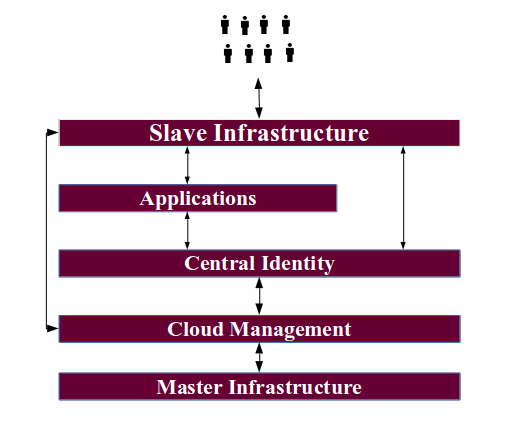
\includegraphics[height=6cm]{./idea.png} \\
 Fig 1. Archtitecture 
\end{figure}
\end{frame}

\begin{frame}{Architecture Continued...}
\begin{figure}[H]
 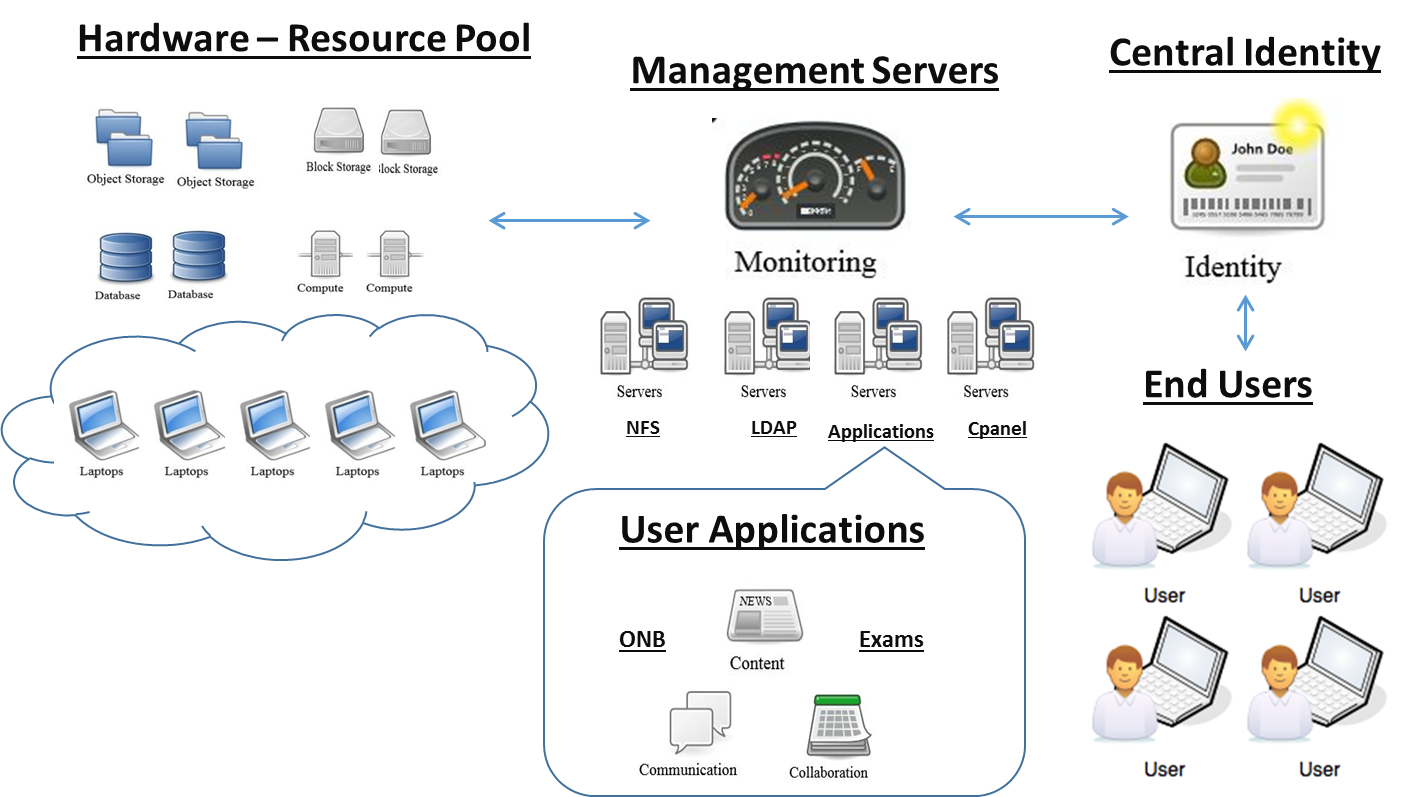
\includegraphics[height=6cm]{./all.png} \\ 
 Fig 2. Archtitecture in detail
\end{figure}
\end{frame}

\section{Proposed System}
\begin{frame}{Proposed System}
\begin{itemize}
	\item Cloud based hardware resources clustering.
	\item Central Identity for all users to access Network based Applicaitons by providing well structured \& documented API.
	\item Dynamic user roles in Central Identity for extended application support.
	\item New CPanel for Network Administration.
		\begin{itemize}
			\item Providing different user modes in OS, controlled remotely from CPanel.
			\item Providing Virtual Labs (machines) with desired resource capabilities.
			\item Providing a right to verify and approve user application requests.
		\end{itemize}
\end{itemize}
\end{frame}

\section{Advantages}
\begin{frame}{Advantages}
\begin{itemize}
	\item Well structured \& controllable Network Administraion
	\item Efficient hardware utilization
	\item No registration for new Network based applications through Central Identity API
	\item Provding Virtual Machines with high hardware configuration for Researchers \& Developers
\end{itemize}
\end{frame}

\section{Implementation...}
\begin{frame}{How to Implement ....}
\begin{itemize}
	\item Why can't we have one Dedicated Lab Environment?
	\item Not only for this project but also to do this kind of projects.
	
\end{itemize}
\end{frame}

\section{New Lab Proposal }
\begin{frame}{New Lab Proposal }
\begin{itemize}
	\item Network and Computational Lab
\end{itemize}
\end{frame}

\section{Requirements}
\begin{frame}{Technical Requirements}
\begin{itemize}
	\item One Lab Envinroment
	\item At Least 10 Computers
	\item Internet facility
		\begin{itemize}
			\item Uninterrupted
			\item No proxy 
			\item Unlimited Data
		\end{itemize}
	\item 24 x 7 Lab availability
\end{itemize}
\end{frame}

\section{Questions?}
\begin{frame}{Questions?}
\centering
Questions and Suggestions? 
\end{frame}


\begin{frame}{Finally ..}
Thank you All .. :)
\end{frame}

\end{document}